\documentclass[a4paper,12pt]{article}
\usepackage[utf8]{inputenc}

%  Русский язык
\usepackage{multirow}
\usepackage{wrapfig}
\usepackage[T2A]{fontenc}			% кодировка
\usepackage[utf8]{inputenc}			% кодировка исходного текста
\usepackage[english,russian]{babel}	% локализация и переносы

\usepackage{indentfirst} %Красная строка
\usepackage[a4paper,top=1.3cm,bottom=2cm,left=1.5cm,right=1.5cm,marginparwidth=0.5cm]{geometry}
\usepackage[usenames]{color}
\usepackage{colortbl}
\usepackage{csvsimple}
\usepackage{siunitx}

\addto\captionsrussian{\def\refname{5   Список используемой литературы}}

% Заметки
\usepackage{todonotes}

% Математика
\usepackage{amsmath,amsfonts,amssymb,amsthm,mathtools} 
\usepackage{hyperref}

\renewcommand{\AA}{\ensuremath{\mathring{A}}}

\begin{document}
\def\figurename{Рисунок}
\begin{titlepage}
\begin{center}
    {\large МОСКОВСКИЙ ФИЗИКО-ТЕХНИЧЕСКИЙ ИНСТИТУТ (НАЦИОНАЛЬНЫЙ ИССЛЕДОВАТЕЛЬСКИЙ УНИВЕРСИТЕТ)}
\end{center}
\begin{center}
    {\largeФизтех-школа биологической и медицинской физики}
\end{center}

\vspace{1cm}
{\huge
\begin{center}
    {\bf Лабораторная работа по физической химии}\\
    \vspace{0.5cm}
    Электрокапиллярные явления
\end{center}
}

\vspace{4cm}
\begin{flushright}
{\LARGE Выполнила студентка группы Б06-103:\\ Фитэль Алена \\}

\end{flushright}
\vspace{9cm}
\begin{center}
    Долгопрудный, 2023 г.
\end{center}
\end{titlepage}
\newpage
\newpage
\section{Введение}
\setcounter{page}{2}
\textbf{Цели работы}: 
\begin{itemize}
	\item Знакомство с потенциометрическими методами определения среднеионных коэффициентов активности электролитов и измерения pH растворов;
	\item Исследование зависимости среднеионного коэффициента активности электролита от его концентрации;
	\item Исследование влияния ионной силы раствора на растворимость солей;
	\item Приобретение практических навыков измерения pH, оценка величины катионной ошибки стеклянного электрода. 
\end{itemize}
\section{Теоретическое введение}
\subsection{Химический потенциал и активности компонентов раствора.}
Для идеального газа(однокомпонентная система) можно получить следующее
выражение для химического потенциала:

\[
\mu(T, p) = \mu^{0}(T) + RT\ln\frac{p}{p^{0}}
\]

Здесь $p$ - давление идеального газа, $p^{0}$ - стандартное давление 1 бар, $ \mu^{0} $ - стандартное значение химического потенциала: $\mu^{0}(T) = \mu(T, p^{0})$.

Химический потенциал компонента идеального раствора:
\[
\mu_{i}(T, p, x) = \mu_{i}^{0}(T, p) + RT\ln x_{i}
\]

где  $\mu_{i}^{0}(T, p) = \mu_{i}(T, p^{0}, x_{i} = 1)$ - стандартный химический потенциал i-го компонента, т.е. его потенциал в "стандартном" состоянии чистого вещества ($x_{i} = 1$) при заданной температуре и давлении $p^{0} = 1 \text{ атм}$. Здесь  $x_{i}$  - мольная доля компонента i.

Химический потерциал для реального раствора:

\[
\mu_{i}(T, p, x) = \mu_{i}^{0}(T, p) + RT\ln a_{i}
\]

Активность i-го компонента, в растворе:

\[
a_{i} = \exp\frac{\mu_{i} - \mu_{i}^{0}}{RT}
\]

Активность $a_{i}$ — безразмерная величина, которая непосредственно выражается через химический потенциал компонента, и не связана напрямую с его концентрацией, хотя и зависит от нее. Это сугубо термодинамическая величина, отражающая вклад компонента в свободную энергию Гиббса раствора:

\[
G(T, p, x) = \sum_{}^{}\nu_{i}\mu_{i} =\sum_{}^{}\nu_{i}(\mu_{i}^{0} + RT\ln a_{i})
\]

Активность можно представить в виде произведения мольной доли компонента $x_{i}$ на его коэффициент активности $\gamma_{i}$:
\[
a_{i} = \gamma_{i}x_{i}
\]
 
Коэффициент активности чистого вещества равен 1. Если $x_{i}\rightarrow1$, то $\gamma_{i} \rightarrow 1$, т.е. $a_{i} \rightarrow c_{i}$. Последнее справедливо, так как когда расстворителя А много, $x_{A} \rightarrow 1 $, то свойства раствора определяются именно растворителем.Для растворенных веществ принимают, что коэффициент активности стремится к единице в бесконечно разбавленном растворе:
\[
 \gamma_{i} \rightarrow 1 \text{ при } x_{i}\rightarrow0,  a_{i} \rightarrow c_{i}
\]

\subsection{Потенциометрическое определение рН}
Величина водородного потенциала рН определяется активностью ионов водорода.
в растворе:
\[
pH = -\lg a_{H^{+}}
\]

Хороший рН-метр по сути является милливольтеметром, с помощью которого проводятся измерения разности потенциалов между электродами, погруженных в раствор Х, которая линейно связана с величиной $pH$ и не зависит от активностей других ионов в исследуемом растворе:

\begin{equation}
    E_{x} = E_{0} - b\cdot pH
\end{equation}


Если данное равентство выполняется то неизвестные коффициенты $E_{0}$, $b$ можно найти на основе калибровки по стандартным буферным растворам. Если концентрация ионов водорода в воде также известна, то можно также выразить коффициент активности ионов водорода:

\[
\gamma_{H^{+}} = \frac{10^{-pH}}{C_{H^{+}}} = \frac{10^{\frac{E_{0}^{st} - E_{x}}{b^{st}}}}{C_{H^{+}}}
\]

Здесь $E_{0}^{st}$, $b^{st}$ обозначают величины, найденные при градуировке(калибровке) по стандартным буферным растворам.

\subsection{ Гальваническая ячейка для измерения рН}

При конструировании цепи для измерения рН необходимо обеспечить независимость потенциала электрода сравнения от состава исследуемого раствора. Например, для этого электроды объединяют в гальваническую ячейку вида:

\begin{figure}[h!]
    \centering
    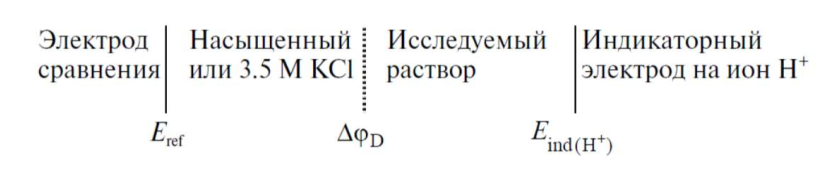
\includegraphics[width = 0.5\textwidth]{1.png}
\end{figure}\\

Исследуемый раствор здесь связан с внутренним раствором $KCl$ хлорсребряного элктрода сравнения через капилляр или пористую мембрану. ЭДС представленной ячейки определяется выражением (следствие уравнения Нернста):
\[
E_{x} = E_{ind} - E_{ref} + \Delta \varphi_{D}
\]
\[
E_{x} = E_{ind}^{0} + \frac{RT}{F}\ln a^{x}_{H^{+}} - (E_{ref}^{0} - \frac{RT}{F}\ln a^{ref}_{Cl^{-}}) + \Delta \varphi_{D}
\]

Преобразуя это выражение, получим, что водородный потенциал в исследуемом
растворе Х выражается через переменную ЭДС цепи $E_{x}$, активность ионов $Cl^{-}$ во внутреннем растворе электрода сравнения, а также зависит от диффузионного потенциала на жидкостных границах:

\[
\lg a^{x}_{H^{+}} + \lg a^{ref}_{Cl^{-}}= \frac{F}{RT\ln 10}(E_{x} + E_{ref}^{0} - E_{ind}^{0} - \Delta \varphi_{D} )
\]

Поскольку активность ионов $Cl^{-}$ во внутреннем растворе электрода сравнения остается постоянной:

\[
pH_{x} \approx \frac{F}{RT\ln 10}(E^{'} - E_{x})
\]

\[
 E_{x} \approx E^{'} - \frac{RT\ln 10}{F}pH_{x}
\]

Это выражение может быть использовано для калибровки по стандартным буфферным растворам.

Есть также другой способ измерения рН раствора в средах с заданной концентрацией хлорид-ионов. Принципильное отличие от предыдущего способа заключается в конструкции гальванической ячейки: индикаторный электрод и электрод сравнения помещаются непосредственно в исследуемый раствор. 
Величина измеряемого напряжения таким электродом будет определяться средней активностью $\sqrt{a_{H^{+}}\cdot a_{Cl^{-}}}$ в растворе:

\begin{equation}
E_{x} = E_{ind} - E_{ref} =  E_{ind}^{0} + \frac{RT}{F}\ln a^{x}_{H^{+}} - (E_{ref}^{0} - \frac{RT}{F}\ln a^{ref}_{Cl^{-}}) = E^{0} + \frac{RT}{F} \ln a_{H^{+}}\cdot a_{Cl^{-}} 
\end{equation}





\subsection{Используемые в работе электроды}
\subsubsection{Стеклянный электрод}
Теория стеклянного электрода исходит из представления о том, что потенциал стеклянного электрода является мембранным потенциалом, возникающем в результате ионообменных свойств стекла. Уравнение, описывающее потенциал стеклянного электрода было получено Б.П. Никольским:
\[
\varphi = \varphi^{0} + \frac{RT}{F}\ln [a_{H^{+}} + K\cdot a_{Na^{+}}]
\]
Если вклад активности ионов $H^{+}$ преобладает над вкладом ионов $Na^{+}$, что выполняется в кислых и нейтральных средах, то имеем:
\[
\varphi \approx \varphi^{0} + \frac{RT}{F}\ln [a_{H^{+}}]
\]
В щелочных средах наблюдается отклонение $E(pH)$ от линейной зависимости - так называемая щелочная ошибка.
Схема устройства стеклянного электрода представленна на Рисунке 1.
\begin{figure}[h!]
    \centering
    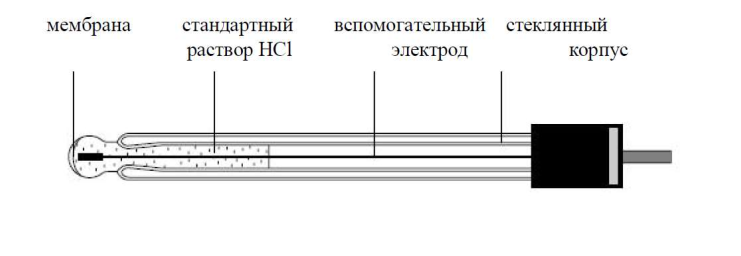
\includegraphics[width = 0.5\textwidth]{2.png}
    \caption{Схема устройства стеклянного электрода}
    \label{fig:no_int}
\end{figure}\\

\subsubsection{Хлорсеребрянный электрод}
Хлорсеребрянный электрод представляет собой тонкую серебрянную проволочку, покрытую слоем труднорастворимой соли $AgCl$ в растворе электролита, содержащего хлорид-ионы.Полуреакция для хлорсеребрянного электрода может быть записана как:
\[
AgCl_{(s)} + e^{-} \rightleftharpoons Ag^{0}_{(s)} + Cl^{-}_{(sol)}
\]
Используя уравнение Нернста и учитывая произведение растворимости $AgCl$ можно показать, что потенциал такого электрода определяется активностью хлорид ионов:
\[
\varphi \approx \varphi^{0} + \frac{RT}{F}\ln a_{Ag^{+}} = \varphi^{0} + \frac{RT}{F}\ln \text{ПР}_{AgCl} - \frac{RT}{F}\ln a_{Cl^{-}} = \varphi^{0}_{2} - \frac{RT}{F}\ln a_{Cl^{-}}
\]

\subsubsection{Комбинированный электрод}

Индикаторный электрод и электрод сравнения могут быть объединены в одну электродную сборку — комбинированный электрод(Рис. 4): 1 — мембрана; 2 —внутренний вспомогательный хлорсеребрянный электрод с раствором $HCl$;  3 — раствор $KCl$; 4 — электролитический ключ для гальванической связи раствора $KCl$ с исследуемым раствором; 5 — электрод сравнения; 6 — стеклянный корпус; 7 — заливочное отверстие электрода сравнения.

\begin{figure}[h!]
    \centering
    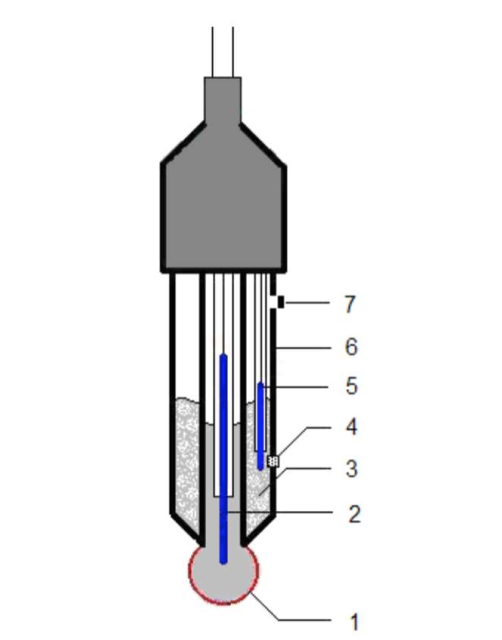
\includegraphics[width = 0.2\textwidth]{4.png}
    \caption{Устройство комбинированного электрода.}
    \label{fig:no_int}
\end{figure}\\


\section{Ход работы и обработка результатов}

\subsection{Калибровка $pH$-метра-иономера}
Проведем каллибровку комбинированного стеклянного электрода по набору стандартных буферных растворов, построим калибровочный график ЭДС в зависимости от $pH$ стандартного буферного раствора. Проведем линейную аппроксимацию полученной зависимости, сравним ее с теоретическим расчетом по формуле (1):
\[
E_{x} = E_{0} - b\cdot pH = 493.5 -59.47 \cdot pH \text{ мВ} \hspace{1cm} b_{teo} = 59 \text{ мВ}
\]

\begin{table}[h!]
\centering
\begin{tabular}{|l|r|r|r|}
\hline
\text{$pH$}                             & 7    & 4,01  & 1,68 \\ \hline
\text{$E, \text{ мВ}$} & 78,4 & 248,4 & 395  \\ \hline
\end{tabular}
\caption{Калибровка рН-метра-иономера}
\label{tab:my-table}
\end{table}

\begin{figure}[h!]
    \centering
    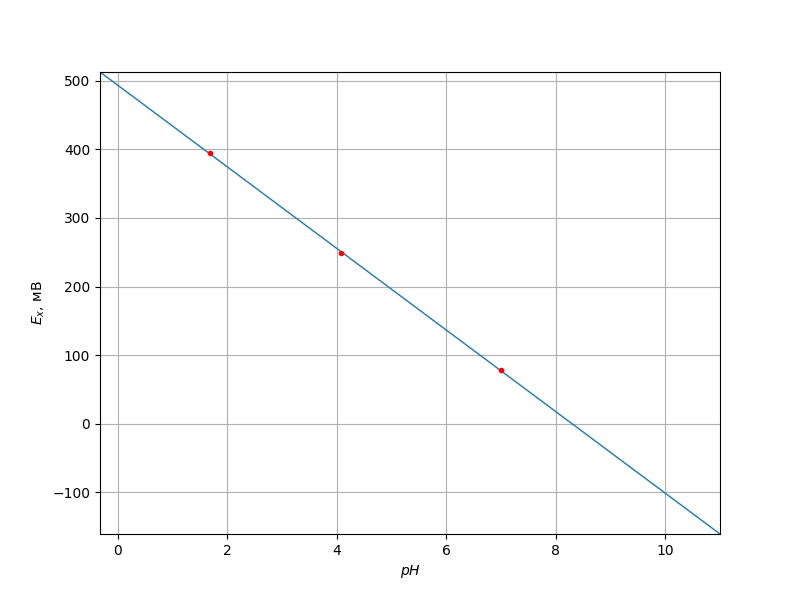
\includegraphics[width=10cm]{Figure_1.png}
    \caption{Калибровка комбинированного электрода}
    \label{fig:vac}
\end{figure}

Далее будем использовать пересчитанное значение напряжения комбинированного стеклянного электрода по полученной зависимости.

\subsection{Определение активности ионов $H^{+}$ и среднеионного коэффициента активноси $HCl$}
\begin{enumerate}
    
\item Проведем измерения ЭДС цепей, состоящих из исследуемого раствора (раствор соляной кислоты в воде) и 1 - комбинированного стеклянного электрода для измерения рН, 2 - стеклянного электрода и хлорсеребряного  электрода сравнения, подключенных к ионометрам, по мере последовательного добавления к ним $2М$ раствора $HCl$. Результаты измерений приведены в Таблице 1.

\begin{table}[h!]
\centering
\begin{tabular}{|r|r|r|r|}
\hline
\multicolumn{1}{|l|}{\textbf{$V_{add}$}} & \textbf{$c_{HCl}$} & \multicolumn{1}{l|}{\textbf{$E_{1}$}} & \textbf{$E_{2}$} \\ \hline
0,1                                       & 0,004               & 344,9                                  & 78,5              \\ \hline
0,4                                       & 0,020                & 385,8                                  & 157,8             \\ \hline
0,5                                       & 0,039               & 402,9                                  & 191,2             \\ \hline
1,0                                         & 0,077               & 420,3                                  & 224,3             \\ \hline
1,0                                         & 0,113               & 429,8                                  & 243,8             \\ \hline
1,0                                         & 0,148               & 437,1                                  & 256,8             \\ \hline
1,0                                         & 0,182               & 442,9                                  & 269,1             \\ \hline
5,0                                         & 0,333               & 457,2                                  & 299,5             \\ \hline
10,0                                        & 0,571               & 469,1                                  & 324,9             \\ \hline
10,0                                        & 0,750                & 475,1                                  & 339,4             \\ \hline
10,0                                        & 0,889               & 478,3                                  & 348,7             \\ \hline
10,0                                        & 1,000                   & 480,6                                  & 355,2             \\ \hline
\end{tabular}
\caption{Результаты измерений ЭДС цепей: 1 - комбинированный электрод, 2 - электрод без жидкостного соединения.}
\label{tab:my-table}
\end{table}

\item Построим графики зависимости ЭДС $E$ от $pC_{H}=-\lg c_{HCl}$. В результате линейных аппроксимаций полученных данных имеем:
\[
E_{1} = -56.64\cdot pC_{H}  + 483.8 \text{ мВ}  \hspace{1cm} E_{2} = -115.30\cdot pC_{H}  + 353.8 \text{ мВ}
\]

\begin{figure}[h!]
    \centering
    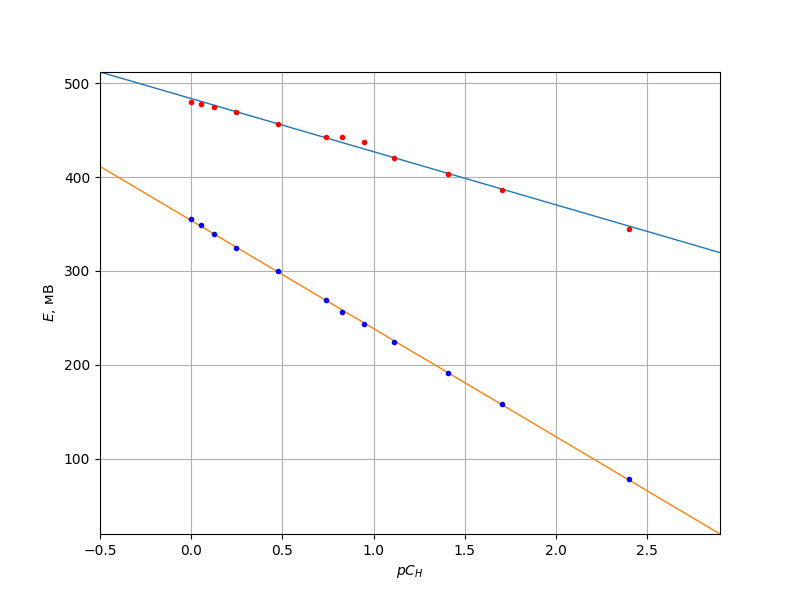
\includegraphics[width=10cm]{Figure_2.png}
    \caption{График зависимости ЭДС $E$ от $pC_{H}=-\lg c_{HCl}$. Синяя прямая - комбинированный электрод, оранжевая – электрод без жидкстного соединения.
}
    \label{fig:vac}
\end{figure}

Наклоны графиков отличаются, так как потенциал электрода с безжидкостным соединением зависит не только от активности $H^{+}$, но и от активности $Cl^{-}$. Причём, активность хлорид-ионов равна активности протонов, следовательно, тангенс угла наклона у прямой электрода с безжидкостным соединением должен быть примерно в 2 раза больше, чем таковой у прямой комбинированного электрода: $\frac{E_{2}^{*0}}{E_{1}^{*0}} = \frac{-115.30}{-56.64} = 2.04 \approx 2$ - экспериментально это подтверждается.

\newpage
\item 
Для серии измерений (2) (с электродом без жидкостного соединения) были расчитаны значения $E^{*} = E - \frac{2RT \ln 10}{F}\lg c_{HCl} + \frac{2RT \ln 10}{F} \cdot \frac{0.51\sqrt{c_{HCl}}}{1 + c_{HCl}}$, которые, согасно третьему приближению теории Дебая-Хюккенса должны равнятся: $E^{*} = E^{0} + \frac{2RT \ln 10}{F} \cdot b \cdot c_{HCl} $. Результаты приведены в Таблице 3.

\begin{table}[h!]
\centering
\begin{tabular}{|r|r|}
\hline
\multicolumn{1}{|l|}{\textbf{$E^{*}$}} & \textbf{$c_{HCl}$} \\ \hline
367,539                                                 & 0,004               \\ \hline
367,960                                                  & 0,020                \\ \hline
368,594                                                 & 0,039               \\ \hline
370,024                                                 & 0,077               \\ \hline
371,657                                                 & 0,113               \\ \hline
372,344                                                 & 0,148               \\ \hline
375,336                                                 & 0,182               \\ \hline
378,484                                                 & 0,333               \\ \hline
379,944                                                 & 0,571               \\ \hline
382,430                                                  & 0,750                \\ \hline
384,236                                                 & 0,889               \\ \hline
385,542                                                 & 1,000                   \\ \hline
\end{tabular}
\caption{Проверка третьего приближения теории Дебая-Хюккенса.}
\label{tab:my-table}
\end{table}

\item Построим линеаризированную зависимость $E^{*}$ от $c_{HCl}$ (Рисунок 3). Используя третье приближение теории Дебая-Хюккеля, экстраполяцией к нулевому значению $c_{HCl}$ найдем значение $E^{0}$ для данной электролитической ячейки:$E^{*} = 17.55 \cdot c_{HCl}  + 369.3 \text{ мВ}$, откуда $E^{0} = 369.3 \text{ мВ}$, $b = 147.5 \frac{\text{ мВ}}{\text{ М}} $. Эмперический параметр $b$ называют константой высаливания.

\begin{figure}[h!]
    \centering
    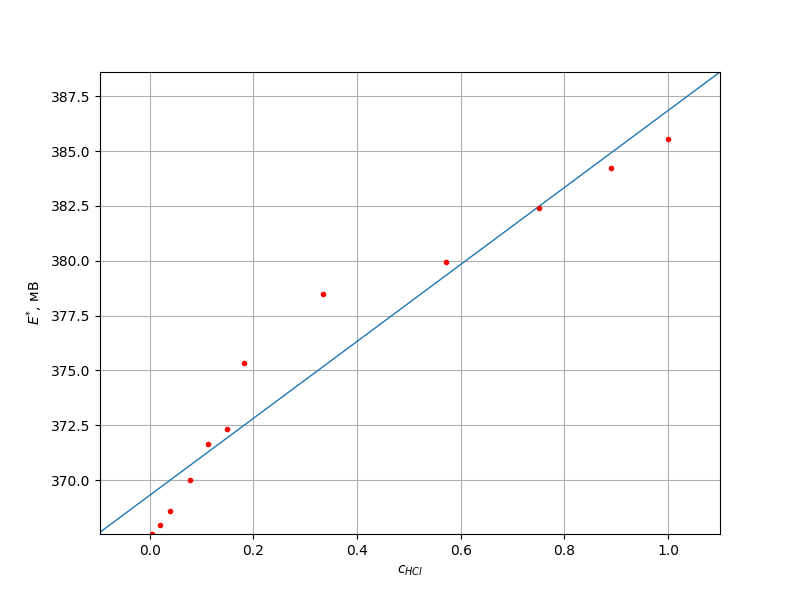
\includegraphics[width=10cm]{Figure_3.png}
    \caption{ График зависимости ЭДС $E^{*}$ от $c_{HCl}$}
    \label{fig:vac}
\end{figure}


\newpage
\item Раcсчитаем коэффициент средней активности раствора $\gamma_{\pm}$ для измерений без жидкостного соединения с помощью найденного значения $E^{0}$, и с помощью проведенной каллибровки расчитаем коэффициент средней активности для комбинированного электрода (Таблица 4). Построим графики зависимости $\lg \gamma_{\pm}$ от квадратного корня из ионной силы раствора $\sqrt{I} = \sqrt{c_{HCl}}$ для двух исследуемых случаев(Рисунок 4).



\begin{table}[h!]
\centering
\begin{tabular}{|r|r|r|}
\hline
\multicolumn{1}{|l|}{\textbf{$\sqrt{c_{HCl}}$}} & \multicolumn{1}{l|}{\textbf{$ \lg \gamma_{pm}^{1}$}} & \multicolumn{1}{l|}{\cellcolor[HTML]{FFFFFF}\textbf{$ \lg \gamma_{pm}^{2}$}} \\ \hline

0,063                                              & -0,045                                                                                             & 1,150                                                                                                                       \\ \hline
0,141                                              & -0,074                                                                                             & 0,811                                                                                                                      \\ \hline
0,198                                              & -0,090                                                                                              & 0,655                                                                                                                      \\ \hline
0,277                                              & -0,105                                                                                             & 0,502                                                                                                                      \\ \hline
0,336                                              & -0,109                                                                                             & 0,414                                                                                                                      \\ \hline
0,385                                              & -0,116                                                                                             & 0,353                                                                                                                      \\ \hline
0,426                                              & -0,102                                                                                             & 0,306                                                                                                                      \\ \hline
0,577                                              & -0,109                                                                                             & 0,168                                                                                                                      \\ \hline
0,756                                              & -0,130                                                                                              & 0,046                                                                                                                      \\ \hline
0,866                                              & -0,126                                                                                             & -0,016                                                                                                                     \\ \hline
0,943                                              & -0,122                                                                                             & -0,055                                                                                                                     \\ \hline
1,000                                                  & -0,118                                                                                             & -0,082                                                                                                                     \\ \hline
\end{tabular}
\caption{Расчет логарифма средних коэффициентов активности растворов для двух электрических ячеек:  1 - комбинированный электрод, 2 - электрод без жидкостного соединения.}
\label{tab:my-table}
\end{table}

\begin{figure}[h!]
    \centering
    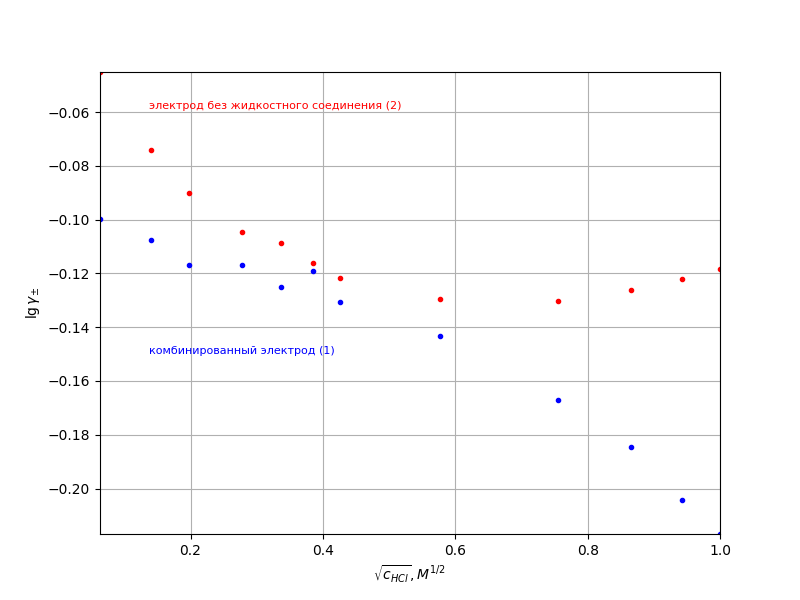
\includegraphics[width=10cm]{Figure_4.png}
    \caption{ График зависимости $\lg \gamma_{\pm}$ от $\sqrt {c_{HCl}}$ для двух электрических ячеек.}
    \label{fig:vac}
\end{figure}

\end{enumerate}

\newpage

\subsection{Определение константы диссоциации уксусной кислоты}
\begin{enumerate}

\item Построим графики зависимости удельной электропроводности уксусной кислоты $\varkappa$ от ее концентрации $c$ и корня из ее концентрации $\sqrt{c}$ по полученным данным(Таблица 5) . Проведем во втором случае линейную аппроксимацию, из которой получим $\varkappa = 1586 \cdot \sqrt{c} + 19.97 \text{ мкСм/см}$. 

\begin{table}[h!]
\centering
\begin{tabular}{|r|r|r|}
\hline
\multicolumn{1}{|l|}{\text{$\varkappa, \text{ мкСм/см}$}} & \multicolumn{1}{l|}{\text{$c$}} & \multicolumn{1}{l|}{\text{$\sqrt{c}$}} \\ \hline
48,1                                                        & 0,001                             & 0,032                                    \\ \hline
292,2                                                       & 0,028                             & 0,167                                    \\ \hline
524,0                                                         & 0,091                             & 0,302                                    \\ \hline
716,0                                                         & 0,191                             & 0,437                                    \\ \hline
1128,0                                                       & 0,500                               & 0,707                                    \\ \hline
\end{tabular}
\caption{Зависимость удельной электропроводности уксусной кислоты $\varkappa$ от ее концентрации $c$ и корня из ее концентрации $\sqrt{c}$.}
\label{tab:my-table}
\end{table}

\begin{figure}[h!]
    \centering
    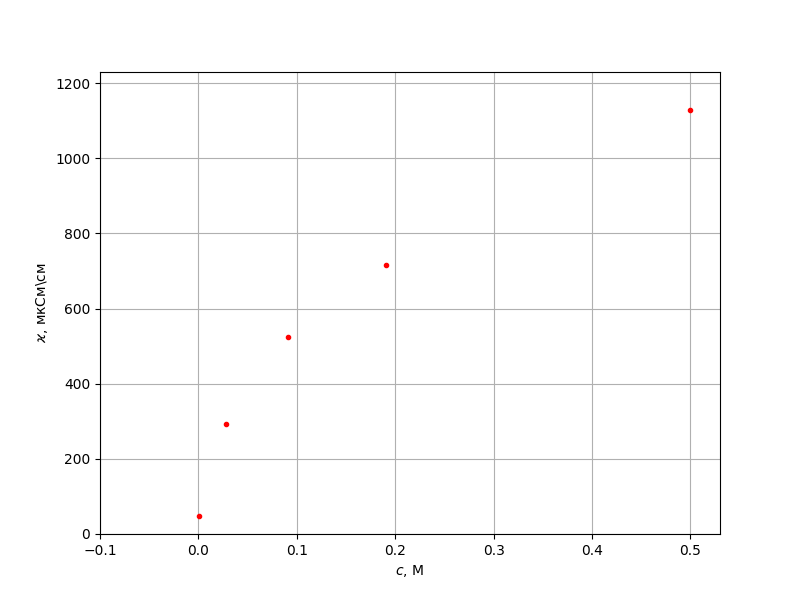
\includegraphics[width=10cm]{Figure_5.png}
    \caption{ График зависимости $\varkappa$ от $c$.}
    \label{fig:vac}
\end{figure}

\begin{figure}[h!]
    \centering
    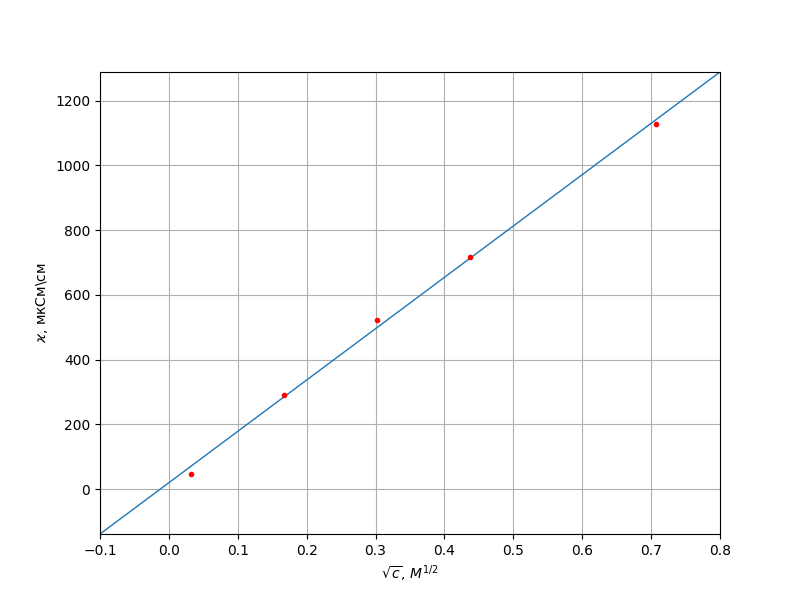
\includegraphics[width=10cm]{Figure_6.png}
    \caption{ График зависимости $\varkappa$ от $\sqrt{c}$.}
    \label{fig:vac}
\end{figure}

\item Константу диссоциации уксусной кислоты рассчитаем из закона разбавления Оствальда и формулы удельной электропроводности:
\[
K = \alpha^{2}c \hspace{1 cm} \varkappa = \lambda c = \alpha \lambda^{0}c =  \lambda^{0} \sqrt{Kc}
 \]

Полученное значение: $K_{a} = = 1.86 \cdot 10^{-5} \text{M}$. Сравним это значение с полученным из графика
зависимости $\varkappa$ от $\sqrt{c}$ (Рисунок 6): коэффициент наклона $k = 1586 =  \lambda^{0} \sqrt{K}$, откуда \cite{1}:
\[
\lambda^{0} = \lambda^{0}_{CH3COO^{-}} + \lambda^{0}_{H^{+}} = 40.9 + 349.8 = 390.7\frac{ \text{См} \cdot \text{cм}^{2}}{ \text{моль}}
\]
\[
K_{a} = \left(\frac {k}{\lambda^{0}}\right)^{2} = \left( \frac{1586 \cdot 10^{-3}}{390.7}\right )^{2} = 1.65 \cdot 10^{-5} \text{ M}
\]

Справочное значение:  $K_{a} = 1.74 \cdot 10^{-5} \text{ M}$ \cite{3}.
\end{enumerate}


\section{Обсуждение результатов и выводы}
\begin{itemize}
\item  Была проведена калибровка комбинированного электрода на буферных растворах. Полученный угол наклона  $b = 59.47 \text{ мВ}$  близок к теоретическому $b_{teo} = 59\text{ мВ}$ .
\item   С помощью электродов с двумя разными типами соединений был определен средний коэффициент активности $HCl$. Из полученных результатов можно сделать вывод о том, что в комбинированном электроде, в месте соприкосновения растворов различных концентраций возникает диффузионный потенциал, точное значение которого расчитать не получится, поэтому для определения среднего коэффициента активности электролитов следует использовать некомбенированный электрод без
жидкостного соединения.

\item На некомбенированном электроде была проверена линейность второго слагаемого в третьем приближении теории Дебая-Хюккенса. 

\item Через удельную электропроводность раствора была оценена константа диссоциации уксусной  кислоты:   $K_{a} = 1.65 \cdot 10^{-5} \text{ M}$, что достаточно близко к теоретическому значению  $K_{a}^{teo} = 1.74 \cdot 10^{-5} \text{ M}$ \cite{3}.

\end{itemize}


\newpage

\addcontentsline{toc}{section}{Список используемой литературы}
\begin{thebibliography}{}
    \bibitem{1}  Кафедра общей химии МФТИ -  "Активность и коэффициент активности ионов в растворах, рН-метрия"
    \bibitem{3}  Лурье Ю.Ю., 1971 г.  -  "Справочник по аналитической химии"
\end{thebibliography}








\end{document}
